\documentclass[10pt]{article}

\usepackage[letterpaper,margin=1in]{geometry}
\usepackage[T1]{fontenc}
\usepackage{hyperref}
\usepackage[parfill]{parskip}
\usepackage{amsmath,amsfonts,amssymb,amsthm}
\usepackage{graphicx}
\usepackage{xcolor}

\graphicspath{{./figs/}}


\vspace{-8ex}
\date{}
\begin{document}

\title{\vspace{-1cm}\textbf{\Large{Intuitive Arm Reach}} \\ \Large{Project Formulation} \\ \textbf{\small{ECE496, 2021-22}}\\\vspace{-0.3cm}}
\author{Defne Dilbaz, Pranshu Malik, Prithvi Marwah, Varun Sampat \\\small{\textbf{Supervisor:}} Professor Mireille Broucke \vspace{-3cm}}

\maketitle

\section{Introduction}
We develop intuition for various tasks through experience. Particularly, we learn to reach for objects in the environment during our infancy, wherein to harness the complexity of our high-dimensional bodies, we are guided by proximodistal patterns of freezing and freeing of degrees of freedom (PDFF), i.e., joints that are closer to the body are more active during self-exploratory movement and more distant joints are progressively involved over the stages of sensorimotor development. This suggests that an innate maturational schedule is involved during sensorimotor development. There is also a related hypothesis, called motor-goal babbling, entailing that we learn to control our bodies by exploring the environment through random movements intended to reach random targets. This way, both hypothetical processes, suggest that through such experiences we develop internal models that allow the movement of limbs in a desired way.

Our project aims to utilize and extend the algorithmic models of aforementioned processes to enable a robotic arm to \emph{intuitively} reach points in its reachable space without the need for explicitly calculating inverse kinematics or dynamics. We heavily rely on the work done in \cite{pdff} which describes how such patterns of exploration can emerge spontaneously as the result of stochastic optimization processes, without explicitly encoding a maturational schedule, and how they can eventually lead to learnt reach actions for a robot. Elements of stochastic optimization also mimic motor babbling and, as a part of the project, we will introduce goal babbling to generate training data to sample and extend this learning process to the robot's reachable space. To conveniently learn and encode goal-directed movements of the robot, we use a simplified form of dynamical movement primitives (DMPs) \cite{dmps}, which is detailed in appendix \ref{subsec:appendix_terms_def}. Here we formulate the requirements, objectives, and components of the Reach Task Learning Algorithm (RTLA) which will be a result of this project.

\section{Assumptions, Knowns, and Constraints}
The underlying assumption is that the robot, much like an infant, has not yet learned inverse kinematics yet, but the forward kinematics and dynamics models are known for the purpose of simulation and error feedback during learning. Specifically, given a joint configuration $\mathbf{q} \in \mathbb{R}^N$, we are able to calculate the corresponding end-effector position in the world frame, ${^W}\mathbf{p}_{N} = \mathcal{K}(\mathbf{q}) \in \mathbb{R}^p$, through the forward kinematic function for an $N$-DOF robot operating in $p$-dimensional space. There is also no initial reach trajectory involved in the learning process, and thus the algorithm starts from scratch rather than from a demonstration. Since the aim of the algorithm is to learn \emph{how} to reach to a certain position, similar to \cite{pdff}, we disregard the goal-attractor dynamics portion of DMPs, because then there is nothing to learn anymore, i.e., the system will implicitly converge to the goal without the algorithm learning to do that part. Therefore, our control policy is not the full dynamical system with an attractor, but only a radial basis function network (\ref{eqn:dmp_radial_basis}) that generates accelerations in joint space (\ref{eqn:dmp_theta_to_qdd}). Essentially, many assumptions that are standard in conventional robotics, such as goal being the attractor state and warm starts in optimization, are dropped in this developmental science approach to reduce the number of required \emph{auxiliary hypotheses} for understanding and emulating the characteristics of human learning in robots. Initially during the development phase, we will exclusively consider planar robots, i.e., $p=2$, and limit ourselves to robot with spherical wrists, i.e., arm structures for which the end-effector orientation can be decoupled from its position. During simulation run-time or deployment on a physical robot, we will only measure the end-effector and goal positions in the world frame to evaluate the task completion condition, $||{^W\mathbf{p}_{N}} - {^W}\mathbf{p}_{g}|| < R_c$ where $R_c$ is the convergence radius.

\begin{figure}[ht]
\centering
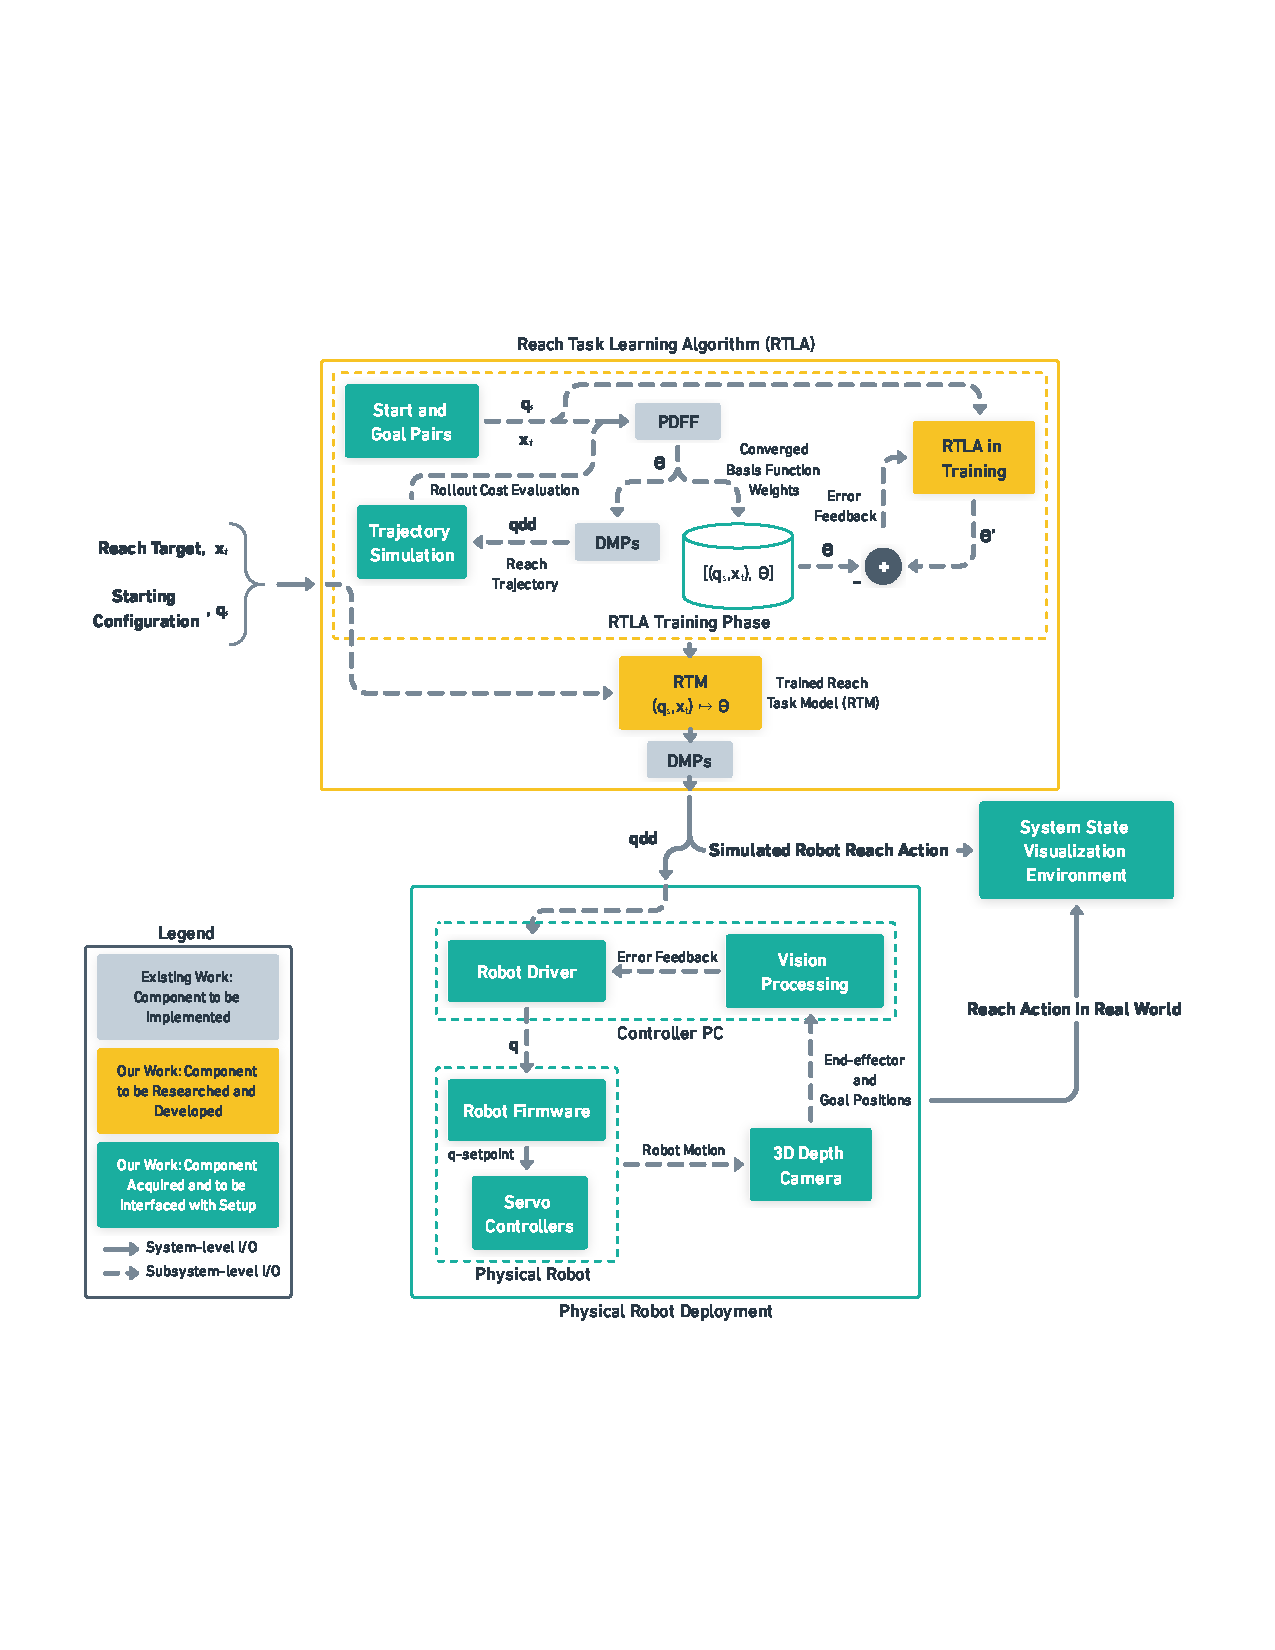
\includegraphics[width=0.7\textwidth]{system_level_overview.pdf}
\label{fig:system_level_overview}
\caption{System level overview}
\end{figure}

\section{Objectives}
We slightly modify the robot arm reach task described above by adding a time-limit $T$ for the reach action, the rationale for which is explained in section \ref{sec:training_algo}. To define the objectives of this task, we borrow the following costs from \cite{pdff} that we would like to minimize together.

\begin{itemize}
	\item \textbf{Reach cost} $||{^W\mathbf{p}_{T, N}} - {^W}\mathbf{p}_{g}||^2$: The squared-distance between the end-effector and the goal positions at the end of the movement ($t = T$). This cost expresses that we want to reach the goal as closely as possible.
	\item\textbf{Comfort cost} $\max(\mathbf{q}_T)$: A cost that corresponds to the largest angle over all  the joints, $1\leq n \leq N$, at the end of the movement. This cost expresses the desire for end-state comfort.
	\item \textbf{Acceleration cost} $r_t$: At each time step $t$, this cost in (\ref{eqn:immediate_cost}) penalizes joint accelerations. The weighting term $(N+1-n)$ penalizes DOFs closer to the origin; the underlying motivation being that wrist movements are less costly than shoulder movements for humans.
\end{itemize}

Thus, we have a terminal cost,

\begin{equation}
\label{eqn:terminal_cost}
	C_T = k_T \cdot \left(||{^W\mathbf{p}_{T, N}} - {^W}\mathbf{p}_{g}||^2 + \max(\mathbf{q}_T)\right)
\end{equation}

and an immediate cost,

\begin{equation}
\label{eqn:immediate_cost}
	r_t  =  k_t \cdot \frac{\sum_{n=1}^N (N+1-n)(\ddot{q}_{t, n})^2}{\sum_{n=1}^N (N+1-n)} \quad .
\end{equation}

Combining, we get the objective function,

\begin{equation}
	\tilde{J}(Q_{\text{dd}}) = C_T\left(\mathcal{K}(\mathbf{q}_T), {^W}\mathbf{p}_{g}, \mathbf{q}_T\right) + \sum_{t=0}^T r_t(\ddot{\mathbf{q}}_t),
\end{equation}

where, $\tilde{J}: \mathbb{R}^{N \times T} \rightarrow \mathbb{R}$ maps the joint accelerations over time, contained in matrix $Q_{\text{dd}}$, to a cost. The overall objective function $J: \mathbb{R}^{B \times N} \rightarrow \mathbb{R}$, accepts parameter matrices $\Theta \in \mathbb{R}^{B \times N}$ from the PDFF algorithm, transforms them to get $Q_{\text{dd}}$ by (\ref{eqn:dmp_theta_to_qdd}), and then returns corresponding costs. We call this process a roll-out, as the parameters directly correspond to the degree of joint accelerations in time and give rise to a reach trajectory that is simulated to then evaluate its quality based on the total cost. Note that the factors $k_T$ and $k_t$ in (\ref{eqn:terminal_cost}) and (\ref{eqn:immediate_cost}) have the purpose of acting as weights for relative prioritization of objectives and to scale and compensate for different ranges of values for the different cost components. For this project, similar to \cite{pdff}, the order of priorities is: reach close to the goal, achieve end-state comfort, and minimize acceleration.

\section{Inputs}
The inertial world frame $W$, the starting configuration $\mathbf{q}_S \in \mathbb{R}^N$, and the goal position ${^W}\mathbf{p}_{g} \in \mathbb{R}^p$ are the only required inputs for RTLA, or $\mathcal{R}_T$.

\section{Outputs}
Given the above inputs, $\mathcal{R}_T$ will output accelerations in the joint space such that for $\mathbf{q}_T = \mathbf{q}_S + \int_0^T\int_0^{T}\ddot{\mathbf{q}}(t)\:dt\:dt$ we have $\mathcal{K}(\mathbf{q}_T) \approx {^W}\mathbf{p}_{g}$, ideally for any goal position in the robot's reachable space. The output $\ddot{\mathbf{q}}(t)$ constitutes the necessary information to carry out the reach action.

\section{Training Algorithm}
\label{sec:training_algo}
As noted before, a key result of \cite{pdff} was that PDFF arises during the stochastic optimization given that we select the above objectives to evaluate the parameters in $\Theta$. Following this study, we also utilize the "Policy Improvement with Black-Box Optimization" ($\text{PI}^{\text{BB}}$) as our stochastic optimization algorithm (section 3.1.4 of \cite{pdff}). During iterative search, once we have a particular $\Theta$, we get the corresponding joint accelerations by the following transformation,

\begin{equation}
\label{eqn:dmp_theta_to_qdd}
        \ddot{\mathbf{q}}^\intercal(t) = \mathbf{g}^\intercal(t)\Theta \quad .
\end{equation}

Here $\mathbf{g}(t) \in \mathbb{R}^B$ is a vector of equally-spaced, time-dependent, and normalized radial-basis functions that together describe the joint space trajectory of each joint when scaled by the respective weights. Note that we constrain the number $B$ for suitable control over joint acceleration profiles. Larger $B$ implies finer control over joint trajectories, but also extra computation in $\text{PI}^{\text{BB}}$. Because of the fixed widths $w$ and center spacing $c_b$ for the basis functions, we have a time bound $T$ for representing the motion of a joint, and hence the reach action. The basis functions are given by,

\begin{equation}
\label{eqn:dmp_radial_basis}
    [\mathbf{g}(t)]_b = \frac{\psi_b(t)}{\sum_{b=1}^{B} \psi_b(t)}, \text{ where } \psi_b(t) = \exp{\left(-\frac{(t-c_b)^2}{w^2}\right)} \quad .
\end{equation}

Note that since $\ddot{\mathbf{q}}$ is a continuous function, we discretize it into timesteps, $t \in [0, T]$. To extend this approach to the robot's reachable space, based on the learnt parameters for training start-goal pairs, we will develop a function approximator, called the Reach Task Model (RTM), that will estimate the parameter matrix $\Theta$ for a given starting pose and goal location, $\mathcal{R}_M: (\mathbf{q}_S, {^W}\mathbf{p}_{g}) \rightarrow \Theta$, such that ${^W}\mathbf{p}_{T,N} \approx {^W}\mathbf{p}_{g}$. This is the main component in the development of $\mathcal{R}_T$ and it operates in a simpler representation than most analytical methods, and hence shows promise for better generalization.

\section{Potential Unique Contributions}
In this project, we attempt to extend and generalize the PDFF-based reach learning method in \cite{pdff} to any robot, including $3-$dimensional multi-jointed arms, and for the entire reachable space, both of which, to our best knowledge, have not been attempted in literature. We have also abstracted the roll-out process for supporting dynamic simulations to get accurate evaluations of joint trajectories for deploying this algorithm on real robots. Lastly, this method has only been implemented in \texttt{MATLAB}, and as a first step, implementing the entire framework using \texttt{Python} and \texttt{C++} is itself a meaningful contribution as it can then be directly applied in real-world use cases.

\section{Extensions and Future Steps}
Currently, this reach-control approach is posed as an open-loop policy during run-time, and assumes perfect transfer to real and simulated robots (with different conditions). This may be corrected for by using vision feedback and a goal-directed formulation, akin to full goal-attractor DMPs, but the main aim of this project is to evaluate generalization of learning in the time-activation representation of joint trajectories. This algorithm will be run on a real robot and in simulation to validate the procedure. Time permitting, we can also test this method for robots with non-spherical wrists, which we initially restricted for simplicity.

\begin{thebibliography}{5}
\bibitem{pdff}
 Stulp, Freek, and Pierre Yves Oudeyer. 2018. “Proximodistal Exploration in Motor Learning as an Emergent Property of Optimization.” Developmental Science 21 (4): 1–12. DOI: \href{https://doi.org/10.1111/desc.12638}{\texttt{10.1111/desc.12638}}.

\bibitem{dmps}
Jan Ijspeert, Auke, Jun Nakanishi, Heiko Hoffmann, Peter Pastor, and Stefan Schaal. n.d. “Dynamical Movement Primitives: Learning Attractor Models for Motor Behaviors.” Relevant  \href{http://www-clmc.usc.edu/Resources/Software}{\texttt{software}}.
\end{thebibliography}

\pagebreak

\appendix
\section*{Appendices}
\addcontentsline{toc}{section}{Appendices}
\renewcommand{\thesubsection}{\Alph{subsection}}
\subsection{Key Terms and Definitions}\label{subsec:appendix_terms_def}

\subsubsection{Dynamical Movement Primitives (DMPs)}
This is a framework that for trajectory planning in dynamical systems for reaching a target state. DMPs enable modeling attractor behaviors of autonomous non-linear dynamical systems with the help of statistical learning techniques. It models a simple dynamical system, defined by a set of linear differential equations, and then transforms them into a weakly nonlinear system with prescribed attractor dynamics by means of a learnable autonomous forcing term. Mathematically, this translates to,

\begin{equation}
    \ddot{y} = \alpha_y(\beta_y(y_g-y) - \dot{y}) + f,
\end{equation}

where $\alpha$ and $\beta$ are gain terms, $y$ is the system state, and $y_g$ is the goal state, and $f$ is the non-linear forcing function that helps achieve the goal and generate the trajectory.

The forcing function $f$ is defined as,

\begin{equation}
    f(x,y_g) = \frac{\Sigma_{b = 1}^{B} \psi_b \theta_b}{\Sigma_{b = 1}^{N} \psi_b}  \cdot x(y_g - y_0),
\end{equation}

where:
\begin{itemize}
	\item $\psi$ is a Gaussian basis function, $\psi_b(x) = \exp\left(-\frac{(x - c_b)^2}{w_b^2}\right)$
	\item $\theta_b$ is the weighting given to its corresponding basis function.
    \item $x$ is defined as the phase of the system with the dynamics $\dot{x} = - \alpha_x x$. Incorporating $x$ into the forcing function ensures that forcing function diminishes to zero over time. 
	\item $y_g - y_0$ is a spatial scaling term, i.e., scaling the activation of each of these basis functions to be relative to the distance to the target, causing the system to cover more or less distance.
\end{itemize}

Essentially, the forcing function arises from a set of weighted Gaussian function, where each Gaussian is located at $c_b$ with variance (or width) $w_b$. These functions parametrize activation over $x$ as the state $y$ converges to its goal $y_g$. As noted in the sections above, we will not be using the goal-attractor canonical system, and instead will only rely on learning the forcing term for each joint as an independent transformation system that takes a parameter vector $\boldsymbol\theta$ and produces a joint acceleration profile.

\end{document}